\subsection{Impulse Response Function}
\textbf{What is an impulse response function?} \\

An impulse response function (IRF) measures the reaction of a time series variable to a shock or impusle at a given point in time.

\begin{figure}[H]
    \centering
    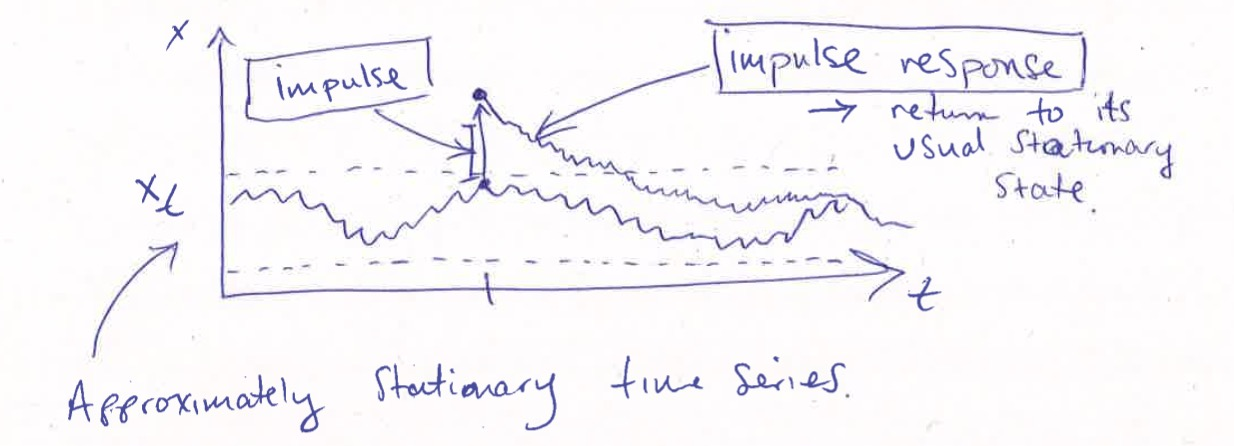
\includegraphics[width=0.8\linewidth]{images/Screenshot 2024-05-21 at 18.13.20.jpg}
    \caption{Impulse Response Function}
\end{figure}


We aim to define the impulse response function IRF(r), wich is related to or equal to: \[
 \text{IRF}(r) = \frac{ \partial X_{t+r} }{ \partial \varepsilon_t }
\]

\textbf{Example: MA(2) Process}\\

Suppose $X_t=\alpha + \varepsilon_t +\theta_1 \varepsilon_{t-1} + \theta_2 \varepsilon_{t-2}$, where:
\begin{itemize}
    \item This is a MA(2) process with parameters $\alpha, \theta_1, \theta_2$
    \item The process is stationary
    \item We can define $X_t$ if we know all $\varepsilon_t$s 
\end{itemize}
The impulse response function for this process can be calculated as follows: 
\begin{align*}
    IRF(r)&=\frac{\partial x_{t+r}}{\partial \varepsilon_t}\\
    IRF(0)&= \frac{\partial(\alpha+\varepsilon_t+\theta_1 \varepsilon_{t-1}+\theta_2 \varepsilon_{t-2})}{\partial \varepsilon_t}\\ 
    &=1\\
    IRF(1)&=\theta_1\\
    IRF(2)&=\theta_2
    \end{align*}

    
\subsubsection{IRFs for More General Models}

Stationary time series are often approximated by moving average (MA) series. Mathematically, a stationary time series can often be represented as an MA($\infty$) series. \\

\textbf{Example: AR(1) Process}\\

Consider an AR(1) model:
    \[
    X_t = \alpha + \rho X_{t-1}+\varepsilon_t
    \]
By inverting the backshift operator $B$, where $X_{t-1} = BX_t$, we get: 
       \[
        X_t= \alpha+\rho BX_t +\varepsilon_t
        \]\[
        \Rightarrow (1-pB)X_t=\alpha+\varepsilon_t
        \]

If $|p|<1$ its possible to invert $(1-pB)$. This is because if the roots of the polynomial in $B$ are outside the unit circle, then we can divide: 
\[
1-\rho B = 0 \longrightarrow B = \frac{1}{\rho} > 1 \text{\quad if} 0<\rho<1
\]

\subsubsection{Inversion and Impulse Response Calculation}

By solving the inversion: \[
(1-\rho B)^{-1}= (1+\rho B + \rho^2 B^2 + \rho^3 B^3 + \cdots
\]
If $X_t$ is sufficiently well-behaved (stationary, etc.) and $|p|<1$, then: 
\[
(1-\rho B)^{-1}X_t= (1+\rho B + \rho^2 B^2 + \rho^3 B^3)X_t
\]\[
(1-\rho B)^{-1} (1-\rho B) X_t = X_t \text{(cancellation property)}\]
Thus: 
\begin{align*}
    X_t &= \alpha+ \rho B X_t + \varepsilon_t\\
    (1-\rho B) X_t &= \alpha + \varepsilon_t \\
    (1-\rho B)^{-1}(1-\rho B) X_t &= (1-\rho B)^{-1} (\alpha + \varepsilon_t)\\
    \Rightarrow X_t &= \alpha + \varepsilon_t + \rho B(\alpha + \varepsilon_t)+ \rho^2 B^2(\alpha+\varepsilon_t) + \cdots
\end{align*}
Now, we can calculate the impulse responses: 
\[
\frac{\partial X_t}{\partial \epsilon_{t-r}}= \frac{\partial}{\partial \epsilon_{t-r}}\rho^r (\alpha + \epsilon_{t-1} )= \frac{\partial}{\partial \epsilon_{t-r}}\rho^r \epsilon_{t-r} = \rho^r
\]
Thus: \[
IRF(r) = \rho^r
\]

\subsubsection{Interpretation}

$\rho^r$ measures the impact of a shock $\varepsilon_t$ at time $t$ on $X_t$ at time $t+r$.

\begin{figure}[H]
    \centering
    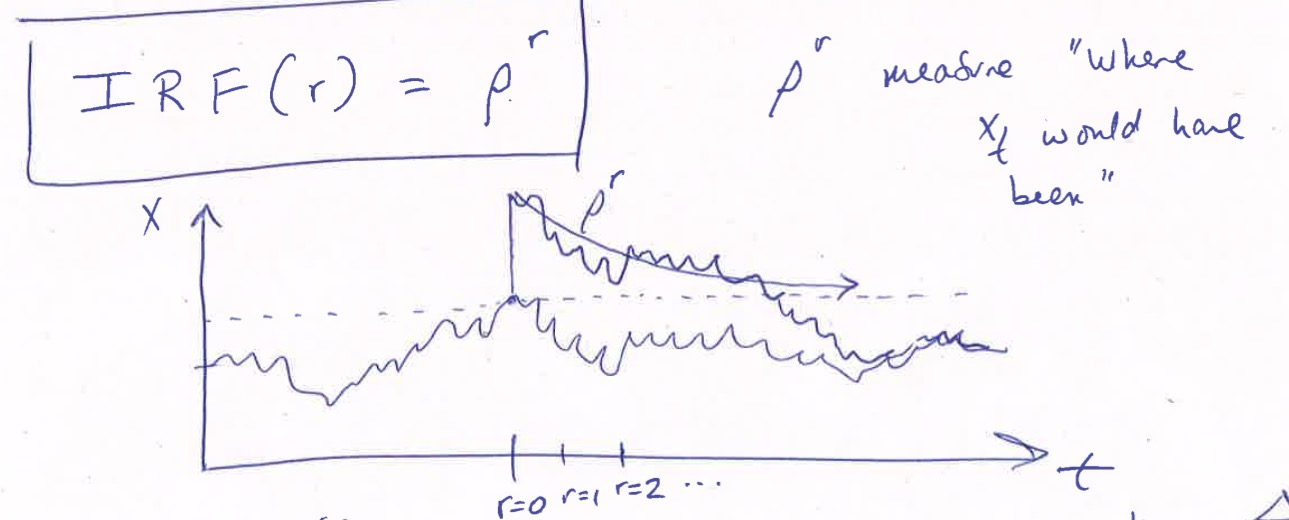
\includegraphics[width=0.75\linewidth]{images/Screenshot 2024-05-21 at 18.16.58.jpg}
\end{figure}

\textbf{MA(2)}

\begin{align*}
    IRF(0) &= 1 \\
    IRF(1)&=\theta_1\\
    IRF(2)&=\theta_2
    \end{align*}
    This tells us:
\begin{itemize}
    \item IRF(0): A shock at time $t$ affects $X_t$ by $1$ unit.
    \item IRF(1): A shock at time $t$ affects $X_{t+1}$ by $\theta_1$.
    \item IRF(2): A shock at time $t$ affects $X_{t+2}$ by $\theta_2$.
\end{itemize}
These values indicate how a shock at time $t$ propagates through the system and affects future values of the time series. \\


\textbf{ARMA(1,1)} \\

\begin{align*}
    X_t &= \alpha + \rho X_{t-1} + \varepsilon_t + \theta \varepsilon_{t-1} \\
    (1-\rho B)X_t &= \alpha + \varepsilon_t + \theta \varepsilon_{t-1} \\
    X_t &= (1-\rho B)^{-1} (\alpha + \varepsilon_t + \theta \varepsilon_{t-1}) \\
&= 1\cdot (\alpha + \varepsilon_t + \theta \varepsilon_{t-1} + \rho B (\alpha + \varepsilon_t + \theta \varepsilon_{t-1}) + \rho^2 B^2(\alpha + \varepsilon_t + \theta\varepsilon_{t-1})
\end{align*}
In this way, we can derive the impulse response function for more complex models.

\subsection{Multivariate Time Series}


\textbf{\underline{Book: Chapter 13}}\\

Observations are often taken simultaneously on two or more time series. For such multivariate data, it may be helpful to develop a multivariate model to describe the interrelationships among the series. However, the model-building process is much more difficult than for univariate models. Multivariate models are more vulnerable to misspecification, this emphasizes the importance of getting sufficient background information so as to understand the context and identify all relevant variables before starting the modelling process. An iterative approach to model building is generally required. With multivariate time series data, the modelling process is complicated by the need to model the serial dependence \textit{within} each series, as well as the interdependence \textit{between} series. Multivariate forecasts are not always as good as might be expected.\\

One basic question is whether the model should involve a single equation or multiple equations. In multiple regression, for example, the model explains the variation in a \textbf{single response} variable in terms of one or more \textbf{predictor} or \textbf{explanatory} variables. In a single-equation model there should not be any suspicion that the response variable could itself affect the predictor variables, i.e., we assume there is an \textbf{open-loop} system. \

When the 'outputs' affect the 'inputs' there is \textbf{feedback} in a \textbf{closed-loop} system, e.g., wages and prices in a simultaneous equation model. \\


\textbf{\underline{Cross-correlation function}}\\

A key tool in modelling multivariate time series is the cross-correlation function. First, look at the bivariate case and the \textbf{cross-variance function} of two time series at the same unit interval and over the same period $(x_1,y_1), \cdots, (x_N, y_N)$, which is defined as \begin{align}
Cov(X_t,Y_{t+k})=\mathbb{E}[(X_t-\mu_x)(Y_{t+k}-\mu_Y)] = \gamma_{XY}(k) \label{cross-cov}
\end{align}
Unlike, the acv.f. this it not an even function. Thus $\gamma_{XY}(k)\neq \gamma_{XY}(-k)$, instead $\gamma_{XY}(k)=\gamma_{YX}(-k)$.\
Useful to standardize the cross-covariance function to produce a function called the \textbf{cross-correlation function}, which is defined as: \[
\rho_{XY}(k)=\frac{\gamma_{XY}(k)}{\sqrt{\gamma_X(0) \gamma_Y(0)}} = \frac{\gamma_{XY}(k)}{\sigma_x \sigma_Y} \label{cross-corr}
\]
\quad where $\sigma_X = \sqrt{\gamma_X(0)}$ denotes the standard deviation of the X-process, and similarly for $\sigma_Y$. This function measures the correlation between $X_t$ and $Y_{t+k}$ and has two properties: 
\begin{enumerate}
    \item $\rho_{XY}(k)= \rho_{YX}(-k)$
    \item $|\rho_{XY}(k)| \leq 1$
\end{enumerate}
Whereas $\rho_X(0), \rho_Y(0)$ are both equal to one, the value of $\rho_{XY}(0)$ is usually \textit{not} equal to one. \\

\begin{equation}
\begin{split}
c_{XY}(k) = & \left\{
\begin{aligned}
    &\sum_{t=1}^{N-k}(x_t-\Bar{x})(y_{t+k}-\Bar{y})/N  &&k=0,1,\cdots, N-1 \\
    & \sum_{t=1-k}^N (x_t-\Bar{x})(y_{t+k}-\Bar{y})/N && k=-1,-2,\cdots,-(N-1)
\end{aligned}
\right.
\end{split}
\end{equation}

and the \textbf{sample cross-correlation function is} \[
r_{XY}(k)= \frac{c_{XY}(k)}{s_X s_Y}
\] \quad where $s_X,s_Y$ are the sample standard deviations.\\
It can be shown that these estimators are asymptotically unbiased and consistent. However, estimators at neighbouring lags are themselves autocorrelated. Furthermore the variances of sample cross-correlations depend on the autocorrelation functions of the two components. In general, the variances will be inflated. Thus it is possible for two series, which are actually uncorrelated, to apparently have large autocorrelation coefficients, which are spurious, in that they arise solely from autocorrelations within the two time series. Solution $\Rightarrow$ one series should first be filtered to convert it to (approximate) white noise and then the same filter is applied to the second series before computing the cross-correlation function.\\

Back to the \textbf{multivariate} case, we redefine the cross-correlation function for an $m$-variate multivariate process, say $\{X_t\}$, where $X_t^T=(X_{1t},X_{2t},\cdots,X_{mt})$. Let $\mu_t$ be the vector of \textbf{mean} values of $X_t$ at time $t$, so that its $i$th component is $\mu_{it}=\mathbb{E}(X_{it})$. Let $\Gamma(t,t+k)$ denote the \textbf{cross-covariance matrix} of $X_t$ and $X_{t+k}$, so that its $(i,j)$th element is the cross-covariance coefficient of $X_{it}$ and $X_{j,t+k}$. A multivariate process is said to be \textbf{second-order stationary} if the mean and the cross-covariance matrices at different lags do not depend on time. Then $\mu_t$ will be a constant, while $\Gamma(t,t+k)$ will be a function of the lag $k$ only, say $\Gamma(k)$. Then the $(i,j)$th element of $\Gamma(k)$, say $\gamma_{ij}(k)$, is given by 
\begin{align}
    \gamma_{ij}(k)=Cov(X_{it},X_{j,t+k})= \mathbb{E}[(X_{it}-\mu_i)(X_{j,t+k}-\mu_j)]
\end{align}
see equation (\ref{cross-cov}). In the stationary case, the set of cross-covariance matrices, $\Gamma(k)$ for $k=0,\pm 1,\pm 2,\cdots$ is called the \textbf{covariance matrix function}. \\
It has rather different properties to the (auto)covariance function in univariate time series in that it is not an even function of lag (as explained above), thus we get \[
\Gamma(k)=\Gamma^T(-k) \quad k=0,\pm1,\pm2,\cdots
\]
Given the covariance matrix function, it is easy to standardize any particular element to find the corresponding cross-correlation and hence construct the set of $(m\times m)$ cross-correlation matrices, $R(k)$ for $k=0,\pm1,\pm2,\cdots$, called the \textbf{correlation matrix function} of the process. Thus the $(i,j)$th element of $R(k)$ is given by 
\begin{align}
    \rho_{ij}(k)=Corr(X_{it},X_{j,t+k})= \frac{\gamma_{ij}(k)}{\sigma_i \sigma_j}
\end{align}
\quad where $\sigma_i$, the standard deviation of $X_{it}$, can also be expressed as $\sqrt{\gamma_{ii}(0)}$.\\

\noindent
\textbf{\underline{Estimation:}} The sample cross-covariance coefficient of $X_i$ and $X_j$ at lag $k$ is given by

\begin{equation}
\begin{split}
c_{ij}(k) = & \left\{
\begin{aligned}
    &\sum_{t=1}^{N-k} (x_{it} - \bar{x}_i)(x_{j,t+k} - \bar{x}_j)/N & \quad & k = 0, 1, \ldots, N-1 \\
    &\sum_{t=1-k}^{N} (x_{it} - \bar{x}_i)(y_{j,t+k} - \bar{x}_j)/N & \quad & k = -1, -2, \ldots, -(N-1)
\end{aligned}
\right.
\end{split}
\end{equation}

and the \textbf{sample cross-correlation coefficient} is given by
\begin{align}
    r_{ij}(k)=\frac{c_{ij}(k)}{s_is_j}
\end{align}
\quad where $s_i=\sqrt{c_{ii}(0)}$ denotes the sample standard deviation of observations on the $i$th variable

\subsubsection{Vector Autoregressive Models}

Vector Autoregressive Models (VAR) are arguably the most important class of models for \textbf{multiple time-series modelling}.\\


\noindent
\textbf{\underline{VAR(1) models}}\\

With $m$ variables, a natural way to represent them is by means of a $(m\times 1)$ vector $\mathbf{X}_t$ where $\mathbf{X}_t^T=(X_{1t},\cdots, X_{mt})$. For simplicity, first look at $m=2$. For stationary series, we may, without loss of generality, assume the variables haven been scaled to have zero mean. 

\begin{equation}
\begin{array}{r@{}l}
& \left.
\begin{aligned}
    X_{1t} &= \phi_{11} X_{1,t-1} + \phi_{12} X_{2,t-1} + \varepsilon_{1t} \\
    X_{2t} &= \phi_{21} X_{1,t-1} + \phi_{22} X_{2,t-1} + \varepsilon_{2t} \label{eq9}
\end{aligned}
\right\}
\end{array}
\end{equation}


where $\phi_{ij}$ are constants. The two 'error' terms $\varepsilon_{1t}$ and $\varepsilon_{2t}$ are usually assumed to be with noise but are often allowed to be correlated contemporaneously. 
\begin{itemize}
    \item If $\phi_{12}=\phi_{21}=0$ then $X_{1t}$ and $X_{2t}$ are not dynamically correlated $\Rightarrow$ univariate case, analyze separately
    \item If one of $\phi_{12}$ and $\phi_{21}$ is not zero, say $\phi_{12}=0$, but $\phi_{21}\neq 0$, then Equation (\ref{eq9}) reduces to
    \begin{equation}
\begin{split}
& \left.
\begin{aligned}
    X_{1t} &= \phi_{11} X_{1,t-1} + \varepsilon_{1t} \\
    X_{2t} &= \phi_{21} X_{1,t-1} + \phi_{22} X_{2,t-1} + \varepsilon_{2t}
\end{aligned}
\right\}
\end{split}
\end{equation}
        \begin{itemize}
            \item In such a case $X_{1t}$ does not depend on the lagged value of $X_{2t}$. Thus, any causality only goes in one direction.
            \item We can think of $X_{1t}$ as the input and $X_{2t}$ as the output. 
        \end{itemize}
\end{itemize}

\noindent
Equation (\ref{eq9}) can be rewritten in vector form as 
\begin{align}
    \mathbf{X}_t=\Phi \mathbf{X}_{t-1}+ \varepsilon_t \label{vectorForm}
\end{align}
where $\varepsilon_t^T=(\varepsilon_{1t},\varepsilon_{2t})$ and \[\Phi=\begin{pmatrix}
    \phi_{11} & \phi_{12}\\
    \phi_{21} & \phi_{22}
\end{pmatrix}\]

\noindent
Equation (\ref{vectorForm}) looks like an AR(1) model except that $\mathbf{X}_t$ (and $\varepsilon_t$) are now vectors instead of scalars. Since $\mathbf{X}_t$ depends on $\mathbf{X}_{t-1}$ we call this model a \textbf{vector autoregressive model} or order 1 (VAR(1)). Equation (\ref{vectorForm}) can further be rewritten as 
\begin{align}
    (I-\Phi B)\mathbf{X}_t =\varepsilon_t \label{13.13}
\end{align}
where $B$ denotes the backward shift operator, $I$ is the ($2\times 2$) identity matrix and $\Phi B$ represents the operator matrix \[\begin{pmatrix}
    \phi_{11}B & \phi_{12}B \\
    \phi_{21}B & \phi_{22}B
\end{pmatrix}\]

The stationarity of $\mathbf{X}_t$ can be extended from the argument for univariate $X_t$. In particular, the necessary and sufficient condition for stationary of (\ref{vectorForm}) or (\ref{13.13}) is that the roots of the determinant of $I-\Phi B$ lie outside the unit circle. \\

The Appendix (\ref{Determinant Calculation }) provides a refresher on how to calculate the determinant of a matrix.\\



\underline{Example Exercise: (13.1)} \\
\begin{footnotesize}
    

\quad Given \begin{align*}
    X_{1t} &= X_{1,t-1}+0.5X_{2,t-1} + \varepsilon_{1t}\\
    X_{2t} &= 0.2 X_{1,t-1} + 0.7 X_{2,t-1} + \varepsilon_{2t}
\end{align*} \quad Is this model stationary and invertible?

\begin{align*}
    X_t &= \begin{pmatrix}
        1 & 0.5 \\
        0.2 & 0.7
    \end{pmatrix}X_{t-1} + \varepsilon_t \\
    \Rightarrow &\text{ VAR(1)} \\
    & \left(I_2 - \begin{pmatrix}
        1 & 0.5 \\
        0.2 & 0.7
    \end{pmatrix}B\right)X_t = \varepsilon_t \\
    \rightarrow &\text{ det}\left(I_2 - \begin{pmatrix}
        1 & 0.5 \\
        0.2 & 0.7
    \end{pmatrix}x\right) \overset{!}{=} 0 \\
    &\text{ det}\begin{pmatrix}
        1-x & -0.5x \\
        -0.2x & 1-0.7x
    \end{pmatrix} \\
    &= (1-x)(1-0.7)-0.1x^2 \\
    &= 1-1.7x + 0.7x^2 -0.1x^2 \\
    &= 1-1.7x + 0.6x^2 \overset{!}{=} 0\\
&\Rightarrow x_1 = \frac{5}{6}, \quad x_2 = 2 \quad \Rightarrow\text{Not stationary}\\
&\text{ As there is no MA component this process is invertible}
\end{align*}

\end{footnotesize}


\noindent
\textbf{\underline{VAR(p) models}}\\

In general a VAR model of order $p$ (order of autoregression) can be written in the form \begin{align}
    \Phi(B) \mathbf{X_t} = \varepsilon_t \label{13.14}
\end{align} where $\mathbf{X}_t$ is a ($m\times 1$) vector of observed variables, and $\Phi$ is a matrix polynomial of order $p$ in the backward shift operator $B$ such that \[
\Phi(B)=I- \Phi_1 B- \cdots - \Phi_p B^p,
\] where $I$ is the ($m\times m$) identity matrix and $\Phi_1, \cdots, \Phi_p$ are ($m\times m$) matrices of parameters. The condition for stationarity is that the roots of the equation \[
\text{determinant}\{\Phi(x)\} = |I-\Phi_1x - \Phi_2 x^2 - \cdots - \Phi_px^p|=0,
\] should lie outside the unit circle.\\

We need to define $m$-dimensional white noise, such as $\varepsilon_t$ in (\ref{13.14}). Let $\varepsilon_t^T=(\varepsilon_{1t},\varepsilon_{2t},\cdots,\varepsilon_{mt})$ denote an ($m \times 1$) vector of random variables. This multivariate time series will be called \textbf{multivariate white noise} if its is stationary with zero mean vector $\mathbf{0}$, and if the values of $\mathbf{\varepsilon}_t$ at different times are uncorrelated. Then the ($m\times m$) matrix of the cross-covariances of the elements of $\mathbf{\varepsilon}_t$ with the elements of $\mathbf{\varepsilon}_{t+j}$ is given by 

\begin{subequations}
\begin{equation}
\begin{array}{r@{}l}
Cov(\mathbf{\varepsilon}_t, \mathbf{\varepsilon}_{t+j}) = & \left\{
\begin{aligned}
    &\Gamma(0) & \quad & j=0 \nonumber \\
    &0_m & \quad & j \neq 0 \nonumber
\end{aligned}
\right.
\end{array}
\end{equation}
\end{subequations}
where $\Gamma_0$ denotes a ($m\times m$) symmetric positive-definite matrix and $0_m$ denotes an ($m \times m$) matrix of zeroes. This means each component of $\mathbf{\varepsilon}_t$ behaves like univariate white noise.\\

Given the matrix $\Gamma_0$, describing the contemporaneous covariances of the white noise, it is possible to evaluate the covariance function, and hence the correlation matrix function of a VAR process (In practice the algebra is horrid). Simple case: One gets a generalized matrix form of the Yule-Walker equations, which can be difficult to solve. Consider, for simplicity VAR(1) model in (\ref{vectorForm}). Multiply through on the right-hand side by $\mathbf{X}_{t-k}^T$ and take expectations. When $k>0$, we get \[
\Gamma(k)=\Gamma(k-1) \Phi^T,
\] but when $k=0$, we get \[
\Gamma(0) =\Gamma(-1)\Phi^T + \Sigma_0 =\Gamma(1)^T \Phi^T + \Sigma_0
\]

\underline{Example Exercise: 13.3}\\

\begin{footnotesize}
Find the covariance matrix function $\Gamma(k)$, and the correlation matrix function $P(k)$ for the VAR(1) model with $\Phi= \begin{pmatrix}
    0.7 & 0\\
    0& 0.3
\end{pmatrix}$, assuming that $\varepsilon_t$ denotes bivariate white noise with covariance matrix $\Gamma_0 = \begin{pmatrix}
    \sigma_1^2 & 0\\
    0& \sigma_2^2
\end{pmatrix}$ at lag zero. \\

\begin{itemize}
    \item The equations are essentially "independent", i.e., no interactions, also \(\varepsilon_{1t}\) and \(\varepsilon_{2t}\) are uncorrelated.
    \item Expectation: \(\text{Cov}_K(X_T)\) is diagonal. (Thus $\Phi \Phi'=\Phi^2$)
\end{itemize}
\begin{align*}
    X_t &= \Phi X_{t-1} + \varepsilon_t \\
\mathbb{E}[X_t X_t'] &= \mathbb{E}[(\Phi X_{t-1} + \varepsilon_t)(\Phi X_{t-1} + \varepsilon_t)']\\
\mathbb{E}[X_t X_t'] &= \Phi \mathbb{E}[X_{t-1} X_{t-1}'] \Phi' + \Phi \mathbb{E}[X_{t-1} \varepsilon_t'] + \mathbb{E}[\varepsilon_t X_{t-1}'] \Phi' + \mathbb{E}[\varepsilon_t \varepsilon_t']\\
\text{Since } \mathbb{E}[X_{t-1} \varepsilon_t'] &= 0 \text{ and } \mathbb{E}[\varepsilon_t X_{t-1}'] = 0: \\
\mathbb{E}[X_t X_t'] &= \Phi E[X_{t-1} X_{t-1}'] \Phi' + \underbrace{E[\varepsilon_t \varepsilon_t']}_{\Gamma_0}\\
\text{Thus } \underbrace{\mathbb{E}[X_tX_t']}_{\Gamma(0)} &= \Phi^2 \underbrace{\mathbb{E}[X_{t-1}X_{t-1}']}_{\Gamma(0)} + \Gamma_0\\
\Rightarrow \Gamma(0) &= \Phi^2 \Gamma(0) + \Gamma_0\\
\Rightarrow \Gamma(0) &= (I- \Phi^2)^{-1} \Gamma_0\\
&= \left(\begin{pmatrix}
    1&0\\
    0&1
\end{pmatrix} - \begin{pmatrix}
    0.49 & 0\\
    0 & 0.09
\end{pmatrix} \right)^{-1} \Gamma_0 \\
&= \begin{pmatrix}
    \frac{\sigma^2_1}{0.51} & 0\\
    0& \frac{\sigma_2^2}{0.91}
\end{pmatrix}\\
 \Gamma(k)&=\Phi^k \Gamma(0)\\
P(k)&=\Phi^k
\end{align*}
\end{footnotesize}


\subsubsection{Vector ARMA Models}

The VAR model may be generalized to include moving average (MA) terms. Building on Equation (\ref{13.14}), this is done by writing \begin{align}
    \Phi (B) \mathbf{X}_t =\Theta(B)\mathbf{\varepsilon}_t
\end{align} where \[
\Theta(B)=I+\Theta_1 B+ \cdots + \Theta_q B^q
\] is a matrix polynomial of order $q$ in the backwards shift operator $B$ and $\Theta_1, \cdots, \Theta_q$ are ($m\times m$) matrices of parameters. Then $\mathbf{X}_t$ is said to follow a \textbf{vector ARMA} (VARMA) model of order $(p,q)$. The \textbf{invertibility condition} is analogous to the univariate case. It requires that the roots of the equation \[ 
\text{determinant}\{\Theta(x)\} =|I+\Theta_1 x + \Theta_2 x^2 + \cdots + \Theta_q x^q|=0
\] should lie outside the unit circle.
 
 \rule{\textwidth}{0.4pt}













\noindent
\textbf{\underline{Lecture:}}\\

Modeling joint dynamics of a multivariate time series.\\
\quad Most common (or basic) approach is to specify a \underline{vector autoregression} \fbox{VAR}.\\

In a bivariate case, $(x_t,y_t) $ two time series
\begin{figure}[H]
    \centering
    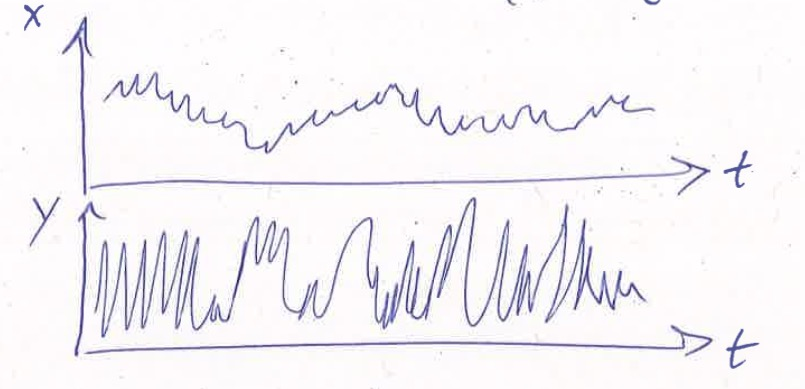
\includegraphics[width=0.75\linewidth]{images/Screenshot 2024-05-21 at 18.18.51.jpg}
\end{figure}

VAR of order 1 is a model of the form: 
\begin{align*}
    y_t&= \alpha+\rho y_{t-1} + \theta x_{t-1} + \varepsilon_t\\
    x_t&= \beta + \xi y_{t-1} + \zeta x_{t-1} + u_t
\end{align*}
Can be written in matrix notation, helpful for more than 2 time series\\

\noindent
Consider $(X_{t,1}, X_{t,2})$ as a bivariate time series. \\
$(X_{t,1}, X_{t,2},\cdots,X_{t,\kappa})$ as a $\kappa$-variate time series. \\

\noindent
Call the vector of observations at time $t$: $X_t$ \\
Similar for $\varepsilon_t$ \\
Then $VAR(1)$ model is written \[
    x_t= \Phi X_{t-1} + \varepsilon_t
\] \quad where $\Phi$ is a matrix

\noindent
\rule{\linewidth}{0.4pt}
\begin{align*}
    \text{If } &y_t = x_{t,1}  \quad x_t = x_{t,2} \ ,\  \Phi = \begin{pmatrix}
\rho & \theta \\
\xi & \zeta 
\end{pmatrix} \\
&\varepsilon_t = \varepsilon_{t,1}  \quad u_t = \varepsilon_{t,2} \\
\text{Then} \\
x_t&= \Phi x_{t-1}+ \varepsilon_t \Leftrightarrow \begin{matrix}
    y_t=\rho y_{t-1} + \theta x_{t-1} + \varepsilon \\
    x_t = \xi y_{t-1} + \zeta x_{t-1} + u_t
\end{matrix}
\end{align*}

Multivariate time series with notation: $X_t = \Phi X_{t-1}  +\varepsilon_t$
\begin{itemize}
    \item Can estimate $\hat{\Phi}$ with maximal likelihood
    \item IRFs - Still problems in defining them
    \begin{itemize}
        \item There are several
        \item For univariate time series we used a MA($\infty$) representation
        \item Will have to take a stand on whether $\varepsilon_{t,1}$ or $\varepsilon_{t,2}$ comes first
        \item There are other alternatives (long run restrictions, ...) 
    \end{itemize}
\end{itemize}
\[
X_t = \Phi X_{t-1} + \varepsilon_t \quad \quad X_t = \begin{pmatrix}
    X_{t,1} \\
    X_{t,2}
\end{pmatrix} ,\ \varepsilon_t = \begin{pmatrix}
    \varepsilon_{t,1}\\
    \varepsilon_{t,2}
\end{pmatrix}
\]
Several impulse response functions:
\begin{align*}
    & \frac{\partial x_{t+r, 1}}{\partial \varepsilon_{t, 1}} & \quad \frac{\partial x_{t+r, 2}}{\partial \varepsilon_{t, 1}} \\
    & \frac{\partial x_{t+r, 1}}{\partial \varepsilon_{t, 2}} & \quad \frac{\partial x_{t+r, 2}}{\partial \varepsilon_{t, 2}}
\end{align*}

\noindent
\rule{\linewidth}{0.4pt}
\noindent
What is a MA($\infty$) for a VAR?\\
Want this to facilitate calculating above 4 listed derivatives.

\begin{align*}
    & \text{Let } B X_t = X_{t-1} \text{ again.} \\
    & B = \begin{pmatrix}
    B_{1-\text{dim}} & 0 \\
    0 & B_{1-\text{dim}}
    \end{pmatrix}
\end{align*}

\[
B \begin{pmatrix}
x_{t,1} \\
x_{t,2}
\end{pmatrix}
= \begin{pmatrix}
B_{1-\text{dim}} x_{t,1} \\
B_{1-\text{dim}} x_{t,2}
\end{pmatrix}
= \begin{pmatrix}
x_{t-1,1} \\
x_{t-1,2}
\end{pmatrix}
\]

\[
(I - \Phi B) x_t = \varepsilon_t
\]

Form \((I - \Phi B)^{-1} \varepsilon_t = X_t\):

\[
X_t = I \varepsilon_t + \Phi B \varepsilon_t + (\Phi B)^2 \varepsilon_t + (\Phi B)^3 \varepsilon_t + \cdots
\]

\subsubsection{Structural VAR}

Unlike standard VAR models from before, \textbf{Structural VAR} (SVAR) models incorporate \textbf{contemporaneous} relationships between variables. This means that the model explicitly captures the effect of the current value of one variable on the current value of another. 

Consider a bivariate SVAR model for two time series $Y_{1t}$ and $Y_{2t}$: 

\begin{equation}
\begin{array}{r@{}l}
& \left.
\begin{aligned}
    Y_{1t} &= a_1 + b_1Y_{2t} + \psi_{11} Y_{1t-1} + \psi_{12} Y_{2t-1} + \varepsilon_{1t} \\
    Y_{2t} &=  a_1 + b_2 Y_{1t} + \psi_{21} Y_{1t-1} + \psi_{22} Y_{2t-1} + \varepsilon_{2t} \label{structural}
\end{aligned}
\right\}
\end{array}
\end{equation}

In this model, $Y_{1t}$ and $Y_{2t}$ can influence each other contemporaneously, represented by the coefficients $b_1$ and $b_2$. This setup allows us to understand and model the immediate effects between variables. This is like a system of equations changing over time. \\

Let
\begin{align*}
    Z_{1t} &= \psi_{11}Y_{1t-1}+\psi_{12}Y_{2t-1} +\varepsilon_{1t} + a_1 \\
    Z_{2t} &= \psi_{21} Y_{1t-1} + \psi_{22} Y_{2t-1} + \varepsilon_{2t} + a_2
\end{align*}
$\Rightarrow$ System 
\begin{subequations}
    \begin{empheq}[box=\fbox]{align*}
    Y_{1t} &= b_1 Y_{2t} + Z_{1t} \\
    Y_{2t}&=b_2 Y_{1t} + Z_{2t}
    \end{empheq}
\end{subequations}

\fbox{$\Rightarrow$ This is like a Model of a moving equilibrium. (moving over $t$)} \\

At each $t$, given $Z_{1t},Z_{2t}$, solve a system to get $Y_{1t}, Y_{2t} $

\begin{figure}[H]
    \centering
    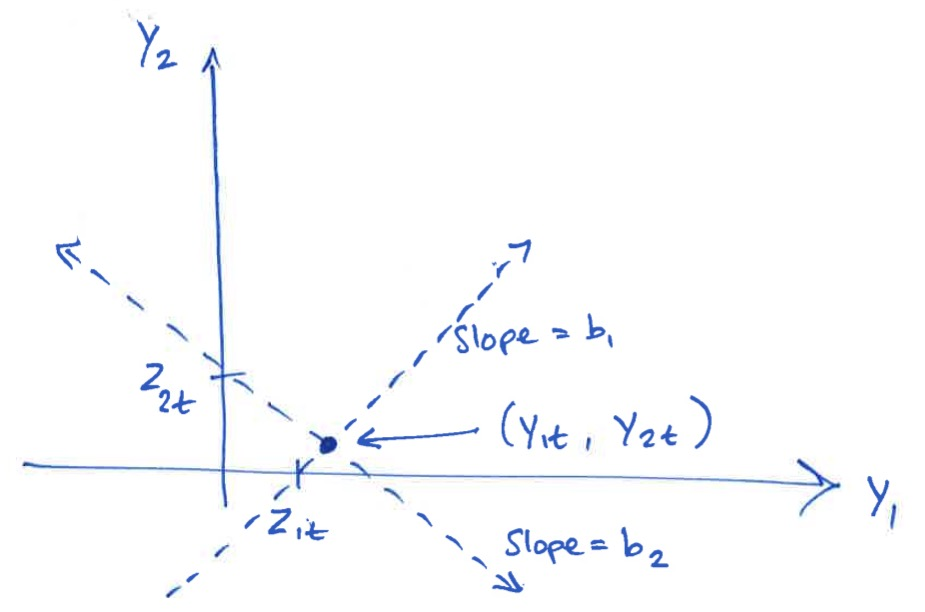
\includegraphics[width=0.5\linewidth]{images/Screenshot 2024-06-08 at 09.12.16.jpg}
\end{figure}

We can derive the corresponding Reduced Form VAR:
\begin{align*}
    Y_{1t} &= \mu_1 + \xi_{11} Y_{1t-1} + \xi_{12} Y_{2t-1} + U_{1t}\\
    Y_{2t} &= \mu_2 + \xi_{21} Y_{1t-1} + \xi_{22} Y_{2t-1} + U_{2t}
\end{align*}
This is simply a VAR model with changed letters. We have no more contemporaneous $Y_{1t}$ or $Y_{2t}$ on the right hand side, the coefficients are now different and residuals are now $U_{t1}$ and $U_{2t}$\\

How does this Reduced Form relate to the Structural Model? 

\begin{align*}
    \text{Let } Y_t = \begin{pmatrix}
        Y_{1t} \\
        Y_{2t}
    \end{pmatrix},\ U_t = \begin{pmatrix}
        U_{1t} \\
        U_{2t}
    \end{pmatrix},\  \varepsilon_t = \begin{pmatrix}
        \varepsilon_{1t}\\
        \varepsilon_{2t}
    \end{pmatrix} \ etc.
\end{align*}

\underline{Structural Model}
\begin{align*}
    Y_t = a + BY_t + \psi Y_{t-1} + \varepsilon_t \quad \text{where } B=\begin{pmatrix}
        0 & b_1  
    \end{pmatrix}
\end{align*}

\underline{Reduced Form Model}
\begin{align*}
    Y_t=\mu + \xi Y_{t-1} + U_t
\end{align*}


In order to relate the two models, we first invert $(I-B)$ from the structural model to get \[
Y_t = (I-B)^{-1} a + (I-B)^{-1} \psi Y_{t-1}+ (I-B)^{-1}\varepsilon_t
\]
This transformation shows that $Y_t$ depends on the past values of $Y_{t-1}$, the structural shocks $\varepsilon_t$, and the coefficients transformed by $(I-B)^{-1}$. The reduced form model is given as $Y_t = \mu + \xi Y_{t-1} + U_t$. To relate this to the structural form, we identify the corresponding terms:
\begin{itemize}
    \item $\mu = (I-BI)^{-1} a$
    \item $\xi = (I-B)^{-1} \psi$
    \item $U_t = (I-B)^{-1} \varepsilon_t$
\end{itemize}

This shows that we can translate between the structural and reduced forms using these transformations. However, there is 1 exception: if the matrix $(I-B)$ is not invertible. \\

The entire purpose is to evaluate how independent shocks to $\varepsilon_{1t}$ and $\varepsilon_{2t}$ of (\ref{structural}) affect the time series. The structure is that $\varepsilon_{1t} \perp \varepsilon_{2t}$, i.e., shocks are assumed to be independent. \[
Cov(\varepsilon_{1t}, \varepsilon_{2t}) = 0
\]
However, in the reduced form \[
Cov(U_{1t},U_{2t})\neq 0
\] So the reduced form and the structural model have a different number of parameters. We thus need to make further assumptions on how $U_t$ relate to $\varepsilon_t$ to make progress on impulse responses or just for estimating $\psi$ or $a$.\\

For that we have many options, we highlight two here:
\begin{itemize}
    \item \textbf{Option 1:} Take a stand on which ($\varepsilon_{1t}$ or $\varepsilon_{2t}$) is first:
    \begin{itemize}
        \item If $\varepsilon_{1t}$ is first, then $\varepsilon_{2t}$ does not directly hit $Y_{1t}$ ($\Rightarrow$ Order shocks and exclude $b_1$)
        \item[] $Y_{1t} = a_1 + 0\cdot Y_{2t} + \cdots + \varepsilon_{1t}$
        \item[] $Y_{2t} = a_2 + b_2 \cdot Y_{1t} + \cdots + \varepsilon_{2t}$
        \begin{itemize}
            \item We can now do recursion (because we set $b_1=0$)
            \item If Shock $\varepsilon_{1t}$ happens we can directly understand what happens to $Y_{1t}$. Then we can think more easily what happens from subsequent $\varepsilon_{2t}$ shock.
        \end{itemize}
        \item \underline{Example:} Currencies
        \begin{itemize}
            \item For instance, in a bivariate model of USD and CHF exchange rates, a shock to the USD will immediately affect the CHF, but a shock to the CHF might take time to impact USD. The order of shocks helps identify immediate and lagged responses accurately 
        \end{itemize}
        \item But now we have to order the shocks to identify IRFs (How? I guess from economic theory)
        \begin{itemize}
            \item How many parameters are there?
            \begin{itemize}
                \item In structural: 9 in total (with $b_1 = 0$ and $Cov(\varepsilon_{1t},\varepsilon_{2t})=0$ restrictions)
                \item In reduced form: also 9 total
                \item $\Rightarrow$ same amount of information in the structural and reduced form models
            \end{itemize}
        \end{itemize}
    \end{itemize}
    \item \textbf{Option 2:} Long-run restrictions:
    \begin{itemize}
        \item Model: $\begin{pmatrix}
            \Delta Y_t \\
            U_t
        \end{pmatrix}$ is stationary + shocks one $\begin{pmatrix}
            e_d \\
            e_s
        \end{pmatrix}$
        \begin{itemize}
            \item $s_0: e_d \perp e_s$ and $e_d$ shocks $\Delta Y_t$, $e_s$ shocks $U_t$
        \end{itemize}
        \item Restriction: In the long run, $e_d$ has no effect on $Y_t$ itself (not differenced) 
        \item Blanchard \& Quad (1986):
        \begin{itemize}
            \item Model $\begin{pmatrix}
                \Delta Y_t \\
                U_t
            \end{pmatrix}$
            \begin{itemize}
                \item where $Y_t$ is output GNP
                \item where $U_t$ is unemployment
            \end{itemize}
            \item In MA representation: 
            \begin{align*}
                \begin{pmatrix}
                    \Delta Y_t \\
                    U_t
                \end{pmatrix} &= \Theta_0 \begin{pmatrix}
                    e_{d_t} \\
                    e_{s_t}
                \end{pmatrix} + \Theta_1 \begin{pmatrix}
                    e_{d_{t-1}} \\
                    e_{s_{t-1}}
                \end{pmatrix} + \Theta_2 \begin{pmatrix}
                    e_{d_{t-2}}\\
                    e_{s_{t-2}}
                \end{pmatrix} + \cdots \\
                \text{Then } &\sum_{i=1}^\infty \left[ \Theta_i \right]_{11} = 0_0 \Rightarrow \text{Identification too}
            \end{align*}
        \end{itemize}
    \end{itemize}
\end{itemize}

\fbox{Key Point: Cannot estimate a structural VAR without at least one economic assumption!}

